\chapter{Experimental Results}
\label{chapter3}
In order to evaluate the algorithm proposed in Chapter~\ref{ch:chapter2} in the context of the Leonardo Drone Contest several experiments where placed. The aim of these experiments was to evaluate the importance of known poles and known and unknown markers in the localization process, the importance of the NEES test to evaluate measurements, the importance of the laser and Octomap measurements, and finally, the accuracy of markers' pose estimation. The whole process was evaluated using ROS bags in order to replicate an experiment with different configurations.\\

Furthermore, the ground truth is provided by a Gazebo plug-in, only in a simulated environment. Odometry only, without correction of any kind, is provided as control process, and used to compare the results. \\

In Figure~\ref{fig:chapter3:odom-only} the control odometry plot is shown. It can be seen the drift in the MAVROS estimate and in the EKF-SLAM estimate. The yaw estimate follows the ground truth with almost no drift in both, MAVROS and EKF-SLAM, estimators, while the drone's height does not follow the ground truth at all in the EKF-SLAM process.\\

It is worth to mention that the negative sign in the Z position of the EKF-SLAM process is due to negative velocities in the control signal. This is not something to be worry about and it is the expected behavior given the linear velocities provided by MAVROS: the positive velocity while the drone takes off is not hold during enough time to position the Z prediction near the ground truth. Furthermore, the linear velocity control signal for the first 25 seconds is negative, which makes the drone "flight below ground". The take off starts at the second 25 and pushes the drone over the ground for some seconds, while the linear velocity published by MAVROS oscillates in between positive and negative values, being the last ones more often. This does not happen with the MAVROS estimator, because it has an own filter that produces the Z position estimation. Hence, the comparison in this case is worthless. The MAVROS EKF filter has nothing to do with the motion model in the EKF-SLAM algorithm which does not correct the prediction in any sense.\\

Less evident is the position estimate in X and Y, where the MAVROS estimation is near the ground truth despite it drifts over time. The EKF-SLAM motion model drifts in a more evident way, both in X and Y: it starts in the same position as the ground truth, and it constantly moves away the control signal. However, and unlike the Z position, both MAVROS and EKF-SLAM motion model follow the ground truth position. Again, comparing the MAVROS estimate with EKF-SLAM prediction is worthless and does not make sense.
\begin{figure}
    \centering
    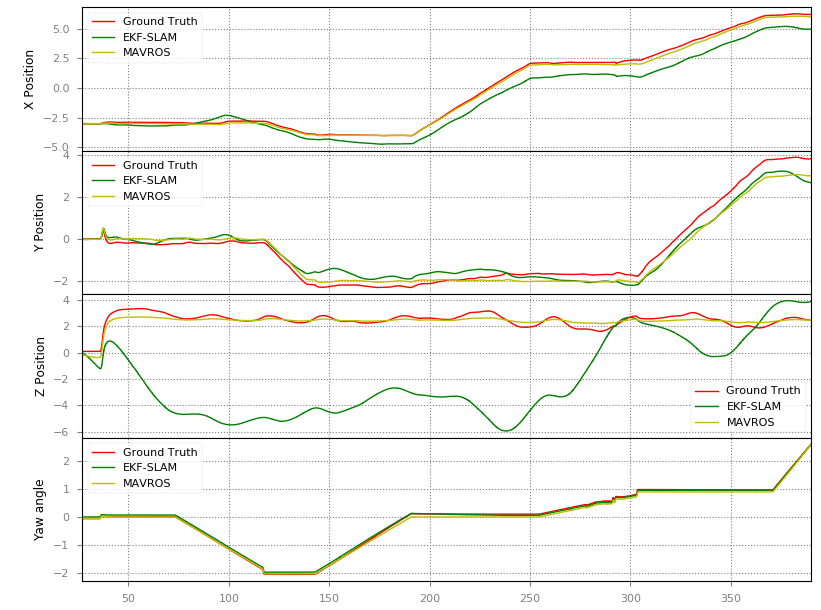
\includegraphics[width=\textwidth]{Images/fig19-odom_only}
    \caption[Odometry only plot]{Odometry only plot. It can be seen three different lines: the red one is the ground truth, the yellow one is the MAVROS estimate and the green one is the EKF-SLAM motion model presented in this work.}
    \label{fig:chapter3:odom-only}
\end{figure}

\section{The Environment}
\label{sec:chapter3:environment}
The simulated environment can be seen in Figure~\ref{fig:chapter3:env:gazebo}, where all the obstacles, poles and markers are disposed. Moreover, the walls define the limits of the environment, making the drone impossible to go off the limits. The markers were disposed arbitrarily around the world, while the poles are in the same place as they should be in the competition: one in each corner, and two along the middle axis of the space.
\begin{figure}
\centering
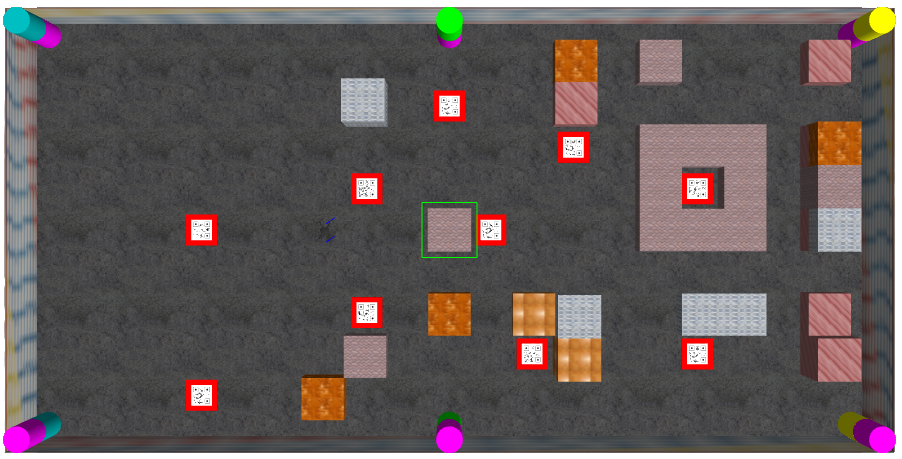
\includegraphics[width=\textwidth]{Images/fig18-gazebo-environment}
\caption{Gazebo simulated environment.}
\label{fig:chapter3:env:gazebo}
\end{figure}
The drone is placed at coordinates $(-3;0)$, and can be depicted in the figure as the green circle in the middle left. As mentioned before, the poles have a different combination of colors, where two poles does not have the same combination. The markers, are QR codes framed in red, while obstacles are brown and gray boxes around the environment. The walls are made of a net-like material distinguishable from the obstacles, while the floor is a pavement-like material.

\section{Simulated Experiments}
\label{sec:chapter3:simulation}

\subsection{Experiment A}
\subsubsection{Procedures}
\label{subsec:chapter3:simulation:procedures}

\subsubsection{Results}
\label{subsec:chapter3:simulation:results}

%\section{Empirical Results ?}
%\label{sec:chapter3:empirical}
%
%\subsection{Procedures}
%\label{subsec:chapter3:empirical:procedures}
%
%\subsection{Results}
%\label{subsec:chapter3:empirical:results}